\section{LLM Judges}
\begin{frame}{}
    \LARGE \textbf{LLM Judges}
\end{frame}

\begin{frame}[allowframebreaks]{LLM Judges: Automatic Semantic Evaluators}

\begin{itemize}
    \item Large Language Models (LLMs) like GPT, LLaMA, and Claude can serve as automatic evaluators, replacing or augmenting human judges for tasks such as translation, summarization, or dialogue evaluation.

    \item How they work:
    \begin{itemize}
        \item Provide the LLM with a reference text (gold standard) and a candidate output (model prediction).  
        \item Supply evaluation instructions or prompts to guide judgment.
    \end{itemize}

    \item Why they are useful:
    \begin{itemize}
        \item LLMs understand meaning and style, not just surface-level word overlap.  
        \item They offer evaluations that are closer to human judgment compared to metrics like BLEU or ROUGE.
    \end{itemize}
\end{itemize}

\begin{figure}
        \centering
        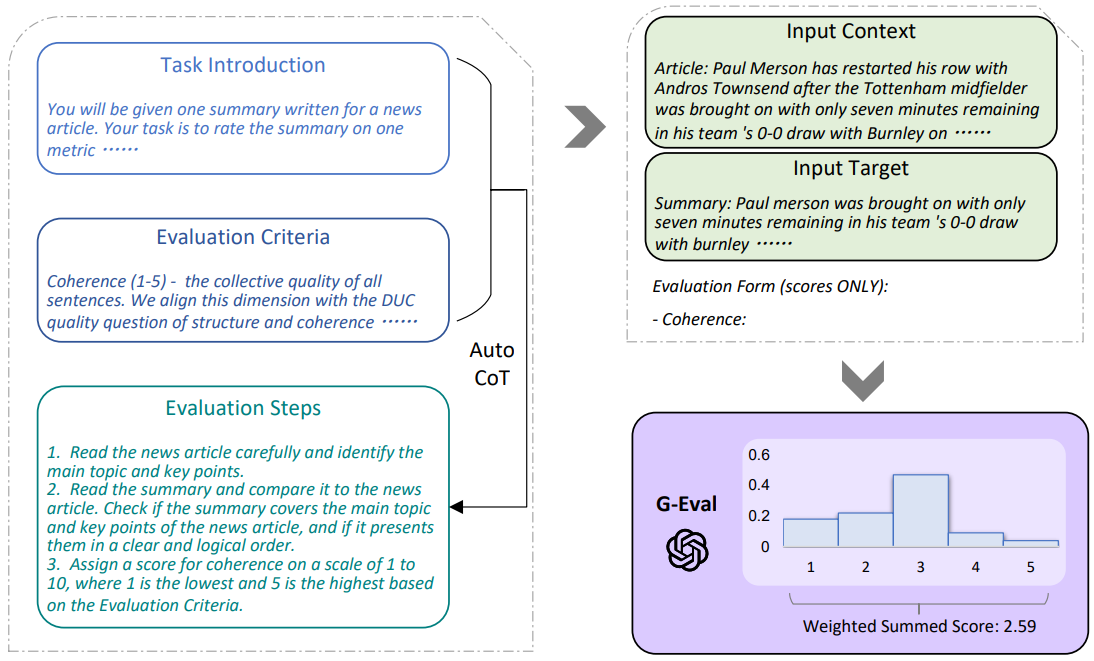
\includegraphics[width=\textwidth,height=0.8\textheight,keepaspectratio]{images/audio-nlp-eval/llm-judges.png}
        \caption*{NLG Evaluation using GPT-4 with Better Human Alignment. Source: \href{https://arxiv.org/abs/2303.16634}{G-Eval}}
    \end{figure}

\end{frame}


\begin{frame}[allowframebreaks]{How LLM Judges Work}

\begin{itemize}
    \item LLMs can automatically evaluate model outputs by comparing them against references using semantic understanding.

    \item Core mechanism:
    \begin{itemize}
        \item \textbf{Prompt design:} Ask the LLM to rate fluency, coherence, and adequacy.  
        Example prompt: ``On a scale of 1–5, how well does Candidate match Reference?''
        \item \textbf{Scoring:} Produce a numeric score or comparative ranking.
        \item \textbf{Calibration:} Aggregate multiple runs to reduce bias and improve consistency.
    \end{itemize}
\framebreak
    \item Conceptual equation:
    \[
        \text{Score}(C, R) = f_\theta(\text{prompt}, C, R)
    \]
    where $f_\theta$ is the LLM evaluating candidate $C$ against reference $R$.

    \item Techniques:
    \begin{itemize}
        \item \textbf{Pointwise:} rate a single candidate.  
        \item \textbf{Pairwise:} compare two candidates, pick the better one.  
        \item \textbf{Listwise:} rank multiple candidates.
    \end{itemize}
\end{itemize}

\end{frame}



\begin{frame}[allowframebreaks]{Why Use LLM Judges?}

\begin{itemize}
    \item Motivation: Traditional metrics and human evaluation have limitations.
    \begin{itemize}
        \item \textbf{N-gram metrics (BLEU/ROUGE):}  \\
        Miss paraphrases  \\
        Ignore fluency and coherence
        \item \textbf{Human evaluation:}  \\
        Reliable  \\
        Expensive and slow
    \end{itemize}

    \item LLM Judges provide a middle ground:
    \begin{itemize}
        \item Understand semantic meaning  
        \item Cheap and scalable  
        \item Flexible across tasks: machine translation, summarization, ASR post-processing
    \end{itemize}
\framebreak
    \item Example:
    \begin{itemize}
        \item Reference: ``The boy is playing soccer.''  
        \item Hypothesis A: ``A child plays football.''  
        \item Hypothesis B: ``The girl eats pizza.''  
        \item BLEU punishes Hypothesis A (word mismatch), but LLM Judge favors A as semantically correct.
    \end{itemize}
\end{itemize}

\end{frame}


\begin{frame}[allowframebreaks]{Use Cases of LLM Judges}

\begin{itemize}
    \item LLM Judges can be applied across multiple NLP and speech tasks:

    \begin{itemize}
        \item \textbf{Machine Translation:} Evaluate adequacy and fluency better than BLEU.  
        \item \textbf{Summarization:} Assess relevance and detect hallucinations.  
        \item \textbf{Dialogue Systems:} Rank chatbot responses (e.g., MT-Bench, Chatbot Arena).  
        \item \textbf{ASR Post-processing:} Rate transcript quality against reference.  
        \item \textbf{TTS/NLG Evaluation:} Measure expressiveness, naturalness, and style.
    \end{itemize}

    \item Example (MT-Bench): GPT-4 performs pairwise comparisons of chatbot responses to select the better reply.
\end{itemize}

\end{frame}


\begin{frame}[allowframebreaks]{Limitations of LLM Judges}

\begin{itemize}
    \item While LLM Judges offer semantic evaluation, they have notable limitations:

    \begin{itemize}
        \item \textbf{Biases:}  
        \begin{itemize}
            \item Position bias: may favor the first candidate.  
            \item Verbosity bias: longer answers can be preferred.  
            \item Self-enhancement: may favor outputs similar to its own style.
        \end{itemize}

        \item \textbf{Stability:} Scores can vary with minor changes in prompt wording.

        \item \textbf{Reproducibility:} LLM outputs are not always deterministic.

        \item \textbf{Transparency:} Evaluation reasoning is often a black-box, making it hard to interpret scores.
    \end{itemize}
\end{itemize}

\end{frame}


\begin{frame}[allowframebreaks]{Best Practices for Using LLM Judges}

\begin{itemize}
    \item To maximize reliability and minimize bias when using LLM Judges:

    \begin{itemize}
        \item Use \textbf{pairwise comparisons} instead of pointwise scoring to reduce bias.  
        \item \textbf{Randomize candidate order} to avoid position bias.  
        \item \textbf{Calibrate} with a small set of human ratings to align scoring.  
        \item Report \textbf{inter-rater reliability} between LLM and human evaluators.  
        \item \textbf{Combine} LLM judgments with traditional metrics (BLEU, ROUGE, WER) for a holistic evaluation.
    \end{itemize}

    \item Why this matters:
    \begin{itemize}
        \item Ensures evaluations are trustworthy, reproducible, and meaningful.
    \end{itemize}
\end{itemize}

\end{frame}
